\section{Appendix \label{sec:AppendixA}}
Figures \ref{fig:HLTJet30IPfirstTrack} to \ref{fig:HLTJet30vertexAnglesMuJets} show a selection of the plots from Sections \ref{sec:impactparameter} to \ref{sec:muonjets} but with a lower trigger threshold  (\verb|HLT_Jet30| in data and \verb|HLTJet15U| in Monte Carlo)  and lower jet momentum cut of $p_t >$ 30 GeV in case of the single jet triggers.  For the b-jet triggers another set of plots has been produced with \verb|HLT_BTagMu_DiJet20_Mu5|, requiring two jets with $p_t >$ 40 GeV, one of them with $p_t >$ 45 GeV.

\begin{figure}[h!]
\centering
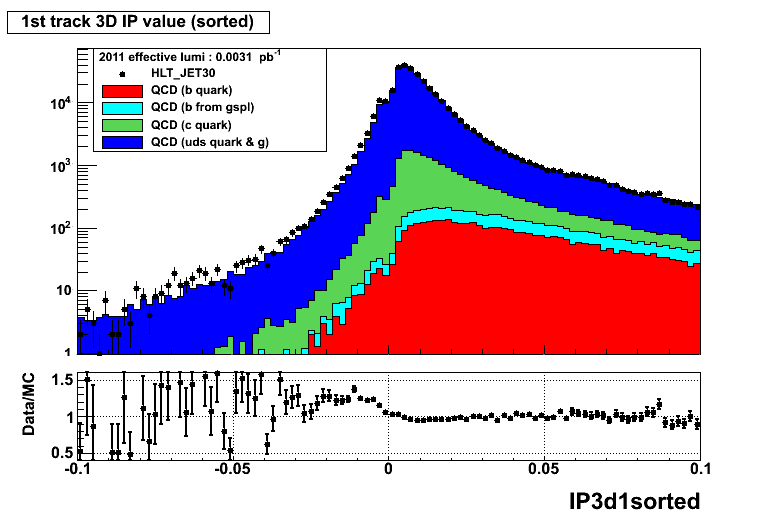
\includegraphics[width=0.32\textwidth]{figures/HLTJet30IP3d1sorted_Log.png}
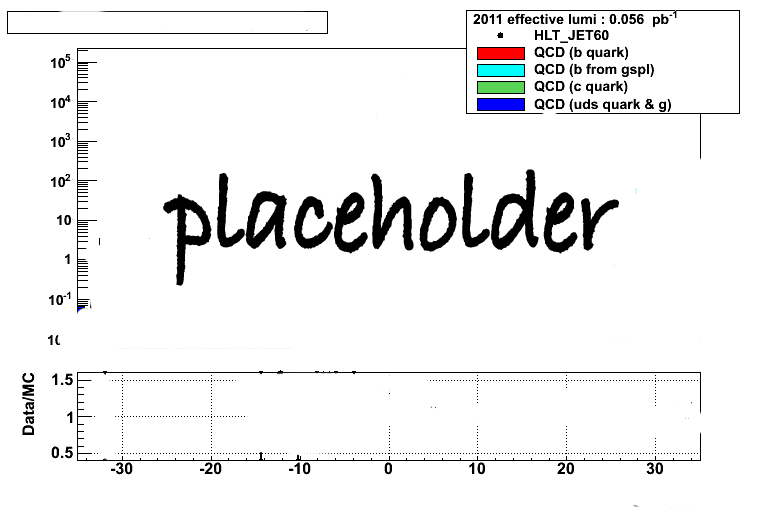
\includegraphics[width=0.32\textwidth]{figures/placeholder.png}
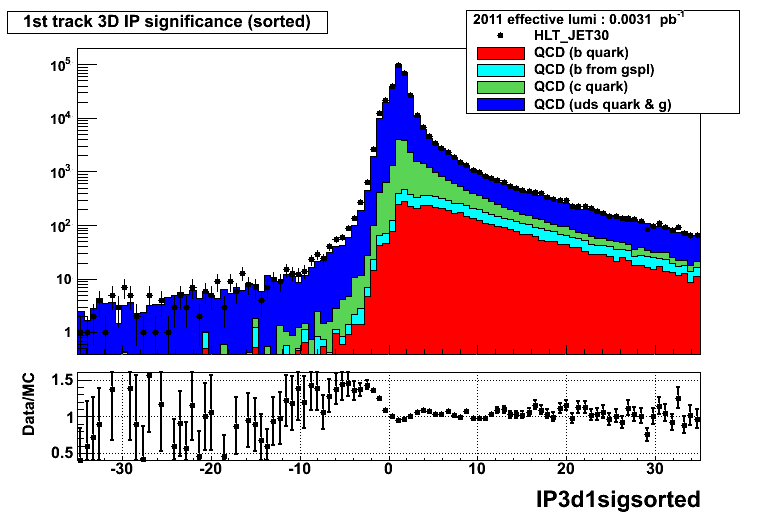
\includegraphics[width=0.32\textwidth]{figures/HLTJet30IP3d1sigsorted_Log.png}
\caption{Left: IP value, middle: IP error, right: IP significance for the first track in the jet, ordered by IP significance.  }
\label{fig:HLTJet30IPfirstTrack}
\end{figure}

\begin{figure}[h!]
\centering
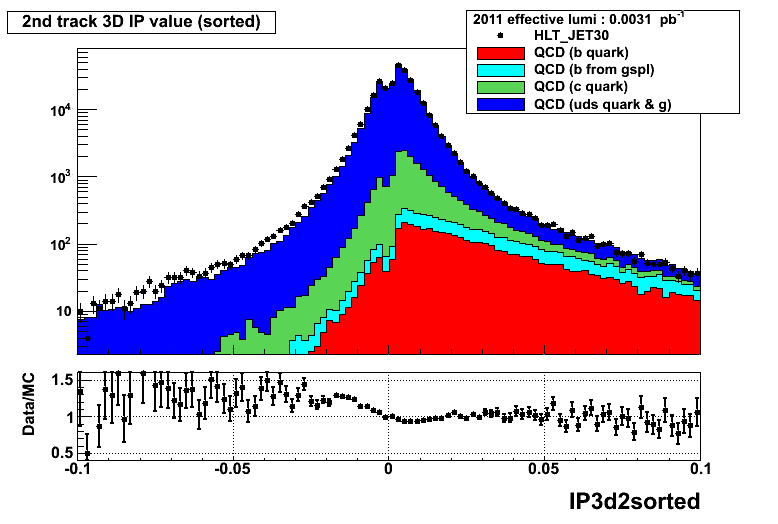
\includegraphics[width=0.32\textwidth]{figures/HLTJet30IP3d2sorted_Log.png}
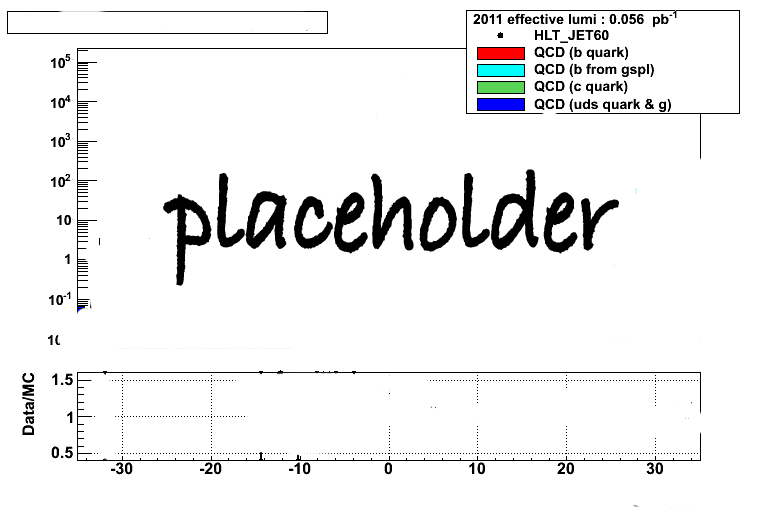
\includegraphics[width=0.32\textwidth]{figures/placeholder.png}
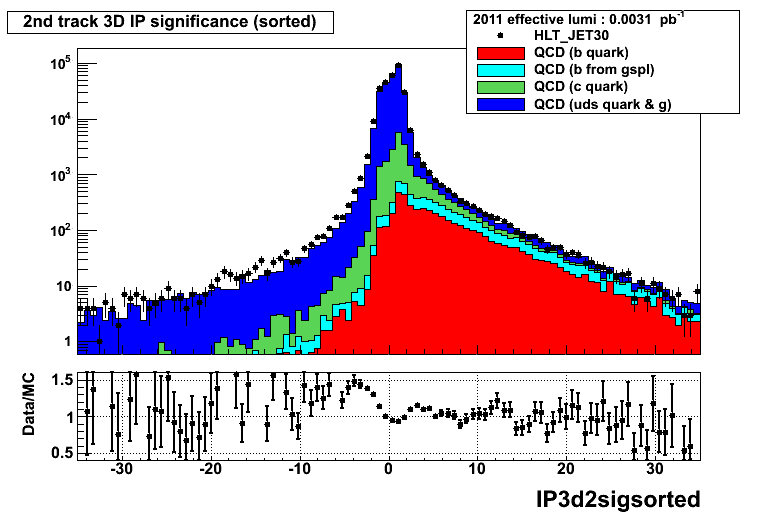
\includegraphics[width=0.32\textwidth]{figures/HLTJet30IP3d2sigsorted_Log.png}
\caption{Left: IP value, middle: IP error, right: IP significance for the second track in the jet, ordered by IP significance.  }
\label{fig:HLTJet30IPsecondTrack}
\end{figure}

\begin{figure}[h!]
\centering
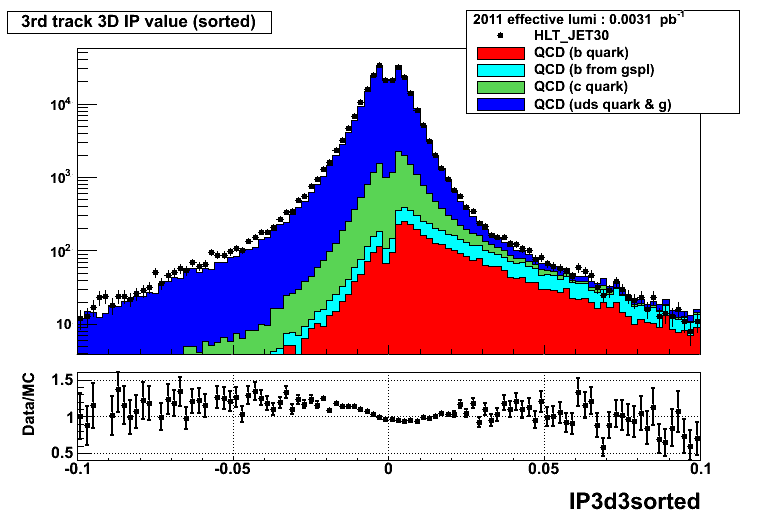
\includegraphics[width=0.32\textwidth]{figures/HLTJet30IP3d3sorted_Log.png}
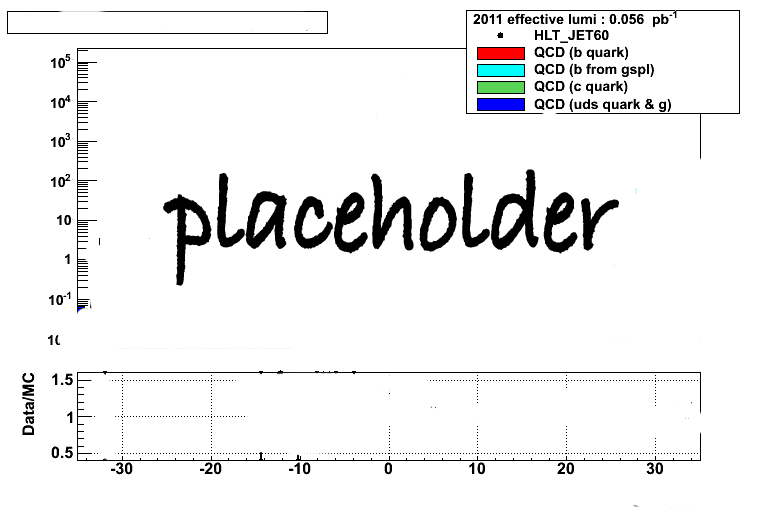
\includegraphics[width=0.32\textwidth]{figures/placeholder.png}
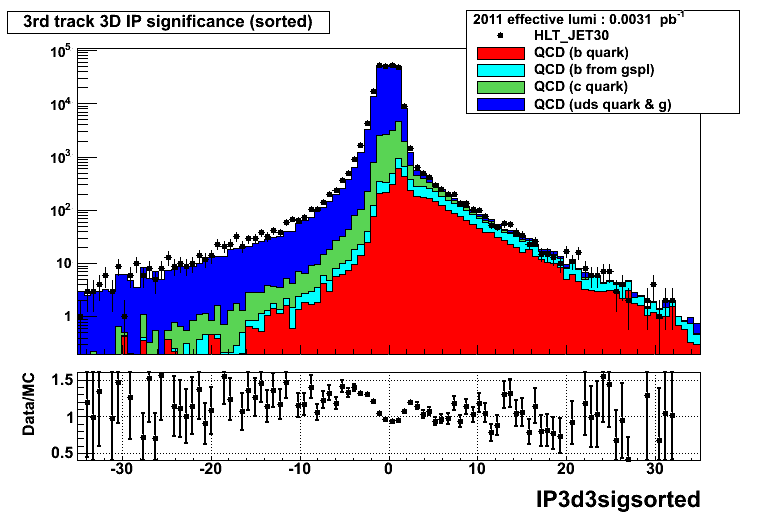
\includegraphics[width=0.32\textwidth]{figures/HLTJet30IP3d3sigsorted_Log.png}
\caption{Left: IP value, middle: IP error, right: IP significance for the third track in the jet, ordered by IP significance.  }
\label{fig:HLTJet30IPThirdTrack}
\end{figure}

\begin{figure}[h!]
\centering
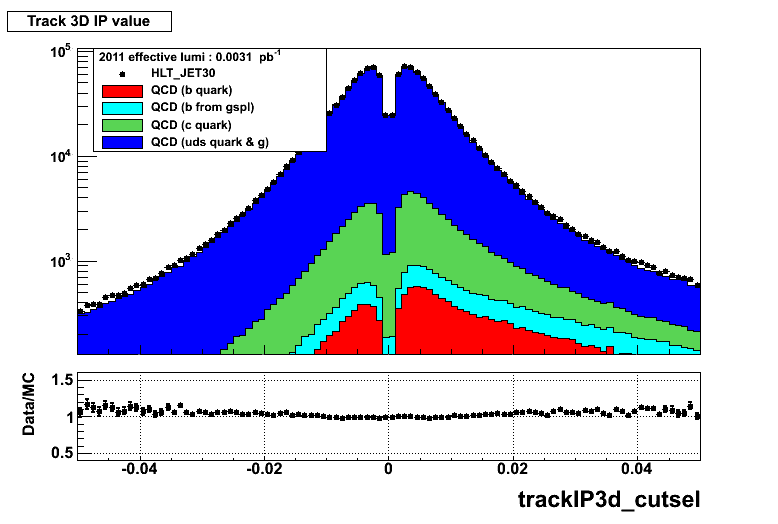
\includegraphics[width=0.32\textwidth]{figures/HLTJet30trackIP3d_cutsel_Log.png}
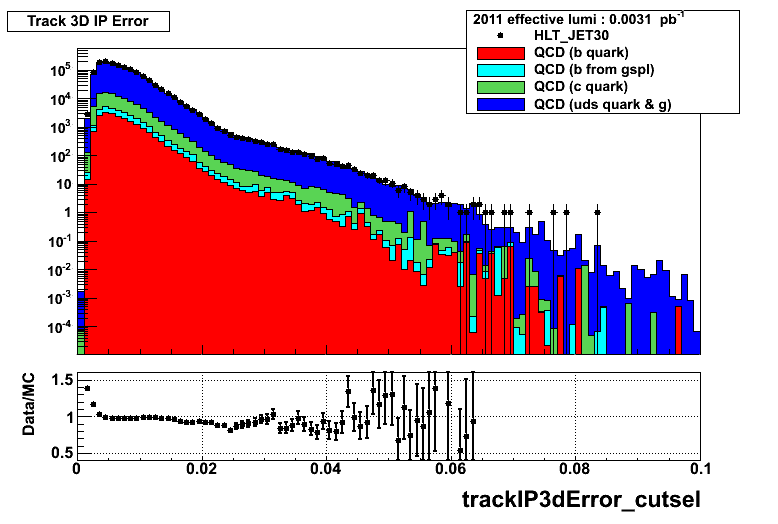
\includegraphics[width=0.32\textwidth]{figures/HLTJet30trackIP3dError_cutsel_Log.png}
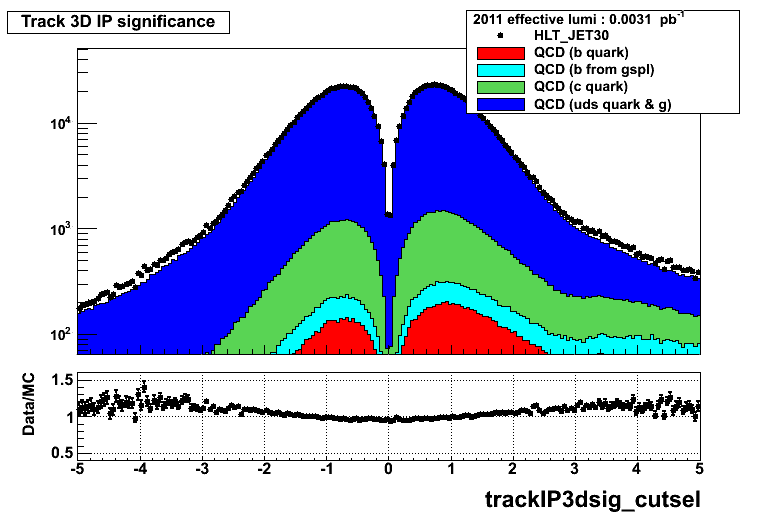
\includegraphics[width=0.32\textwidth]{figures/HLTJet30trackIP3dsig_cutsel_Log.png}
\caption{Left: IP value, middle: IP error, right: IP significance for all selected tracks in the jet. The track selection as defined in Section~\ref{sec:trackselection} has been applied.}
\label{fig:HLTJet30IPAllTrack}
\end{figure}

\begin{figure}[h!]
\centering
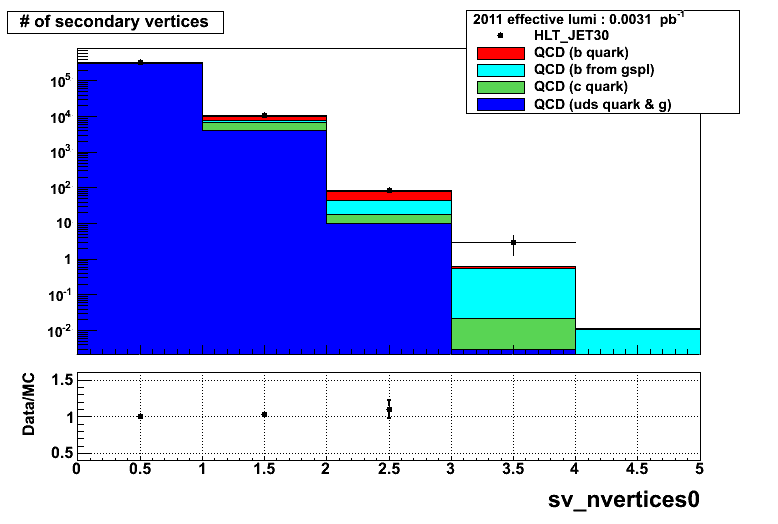
\includegraphics[width=0.32\textwidth]{figures/HLTJet30sv_nvertices0_Log.png}
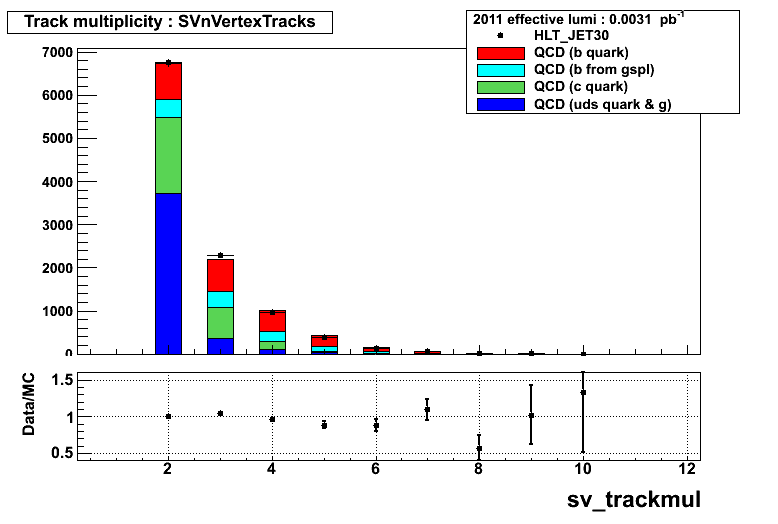
\includegraphics[width=0.32\textwidth]{figures/HLTJet30sv_trackmul_Linear.png}
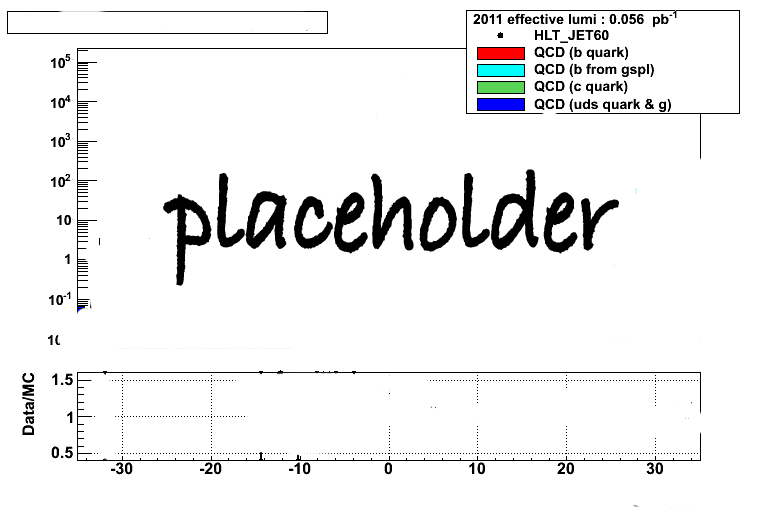
\includegraphics[width=0.32\textwidth]{figures/placeholder.png}
\caption{Left: number of reconstructed secondary vertices per jet, middle: number of tracks at the reconstructed secondary vertex, right: average number of tracks at the secondary vertex versus jet $p_t$. }
\label{fig:HLTJet30vertexNtracks}
\end{figure}

\begin{figure}[h!]
\centering
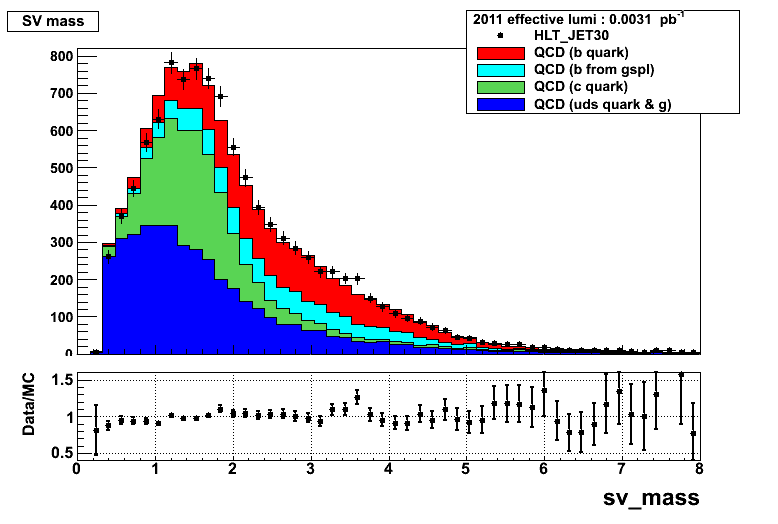
\includegraphics[width=0.32\textwidth]{figures/HLTJet30sv_mass_Linear.png}
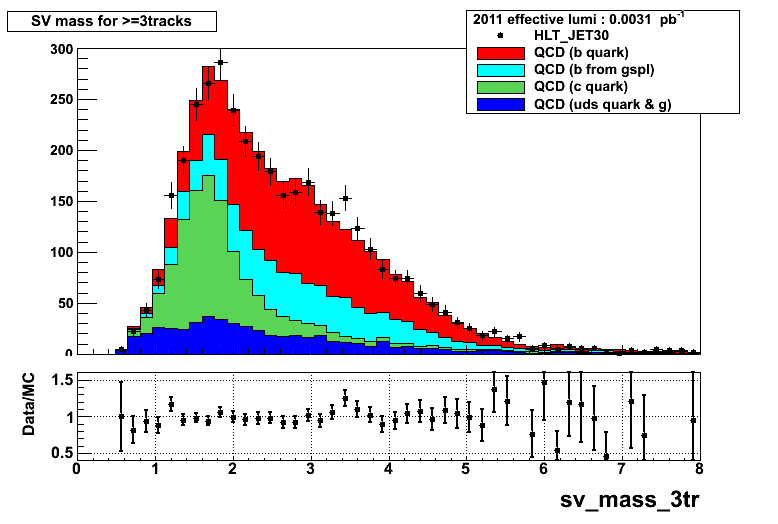
\includegraphics[width=0.32\textwidth]{figures/HLTJet30sv_mass_3tr_Linear.png}
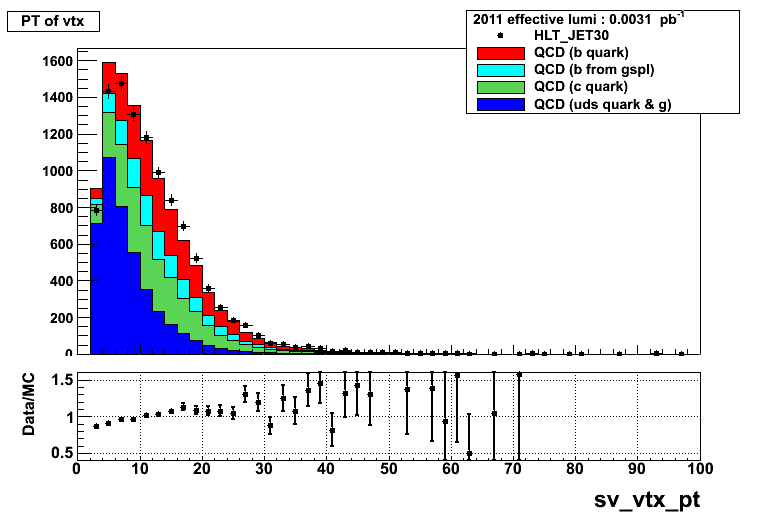
\includegraphics[width=0.32\textwidth]{figures/HLTJet30sv_vtx_pt_Linear.png}
\caption{Left: vertex mass with two or more reconstructed tracks at the vertex. Middle: vertex mass with three or more tracks at the vertex. Right: transverse momentum of the secondary vertex (with two or more tracks). }
\label{fig:HLTJet30vertexMass}
\end{figure}

\begin{figure}[h!]
\centering
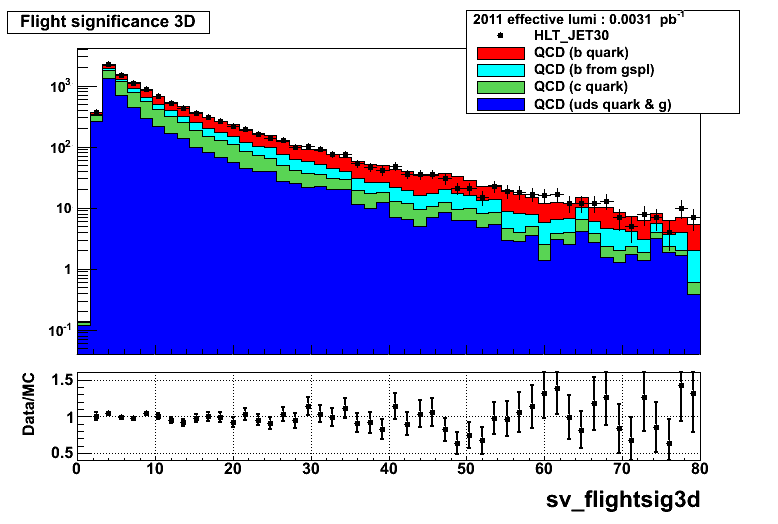
\includegraphics[width=0.32\textwidth]{figures/HLTJet30sv_flightsig3d_Log.png}
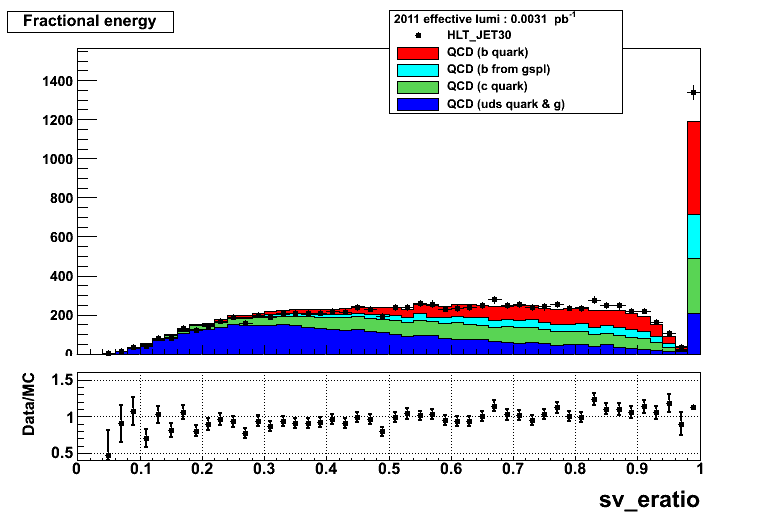
\includegraphics[width=0.32\textwidth]{figures/HLTJet30sv_eratio_Linear.png}
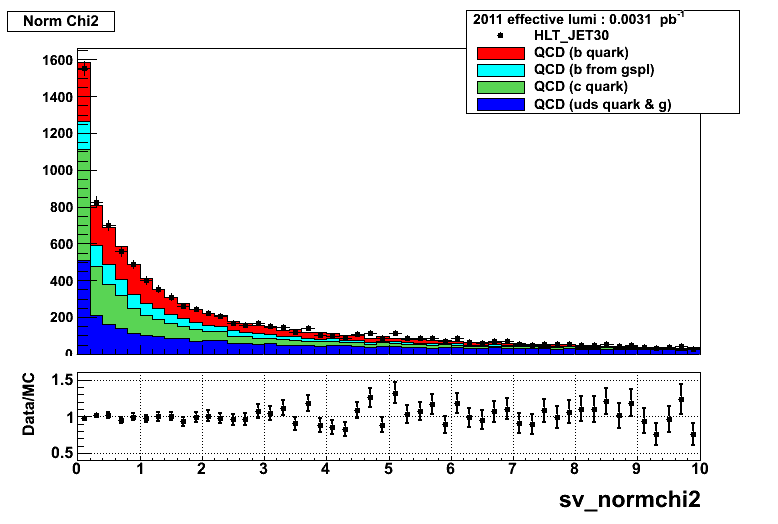
\includegraphics[width=0.32\textwidth]{figures/HLTJet30sv_normchi2_Linear.png}
\caption{Left: vertex flight distance significance. Middle: ratio of track energy at the secondary vertex with respect to all selected tracks in the jet. Right: vertex fit normalized $\chi^2$. }
\label{fig:HLTJet30vertexdistance}
\end{figure}

\begin{figure}[h!]
\centering
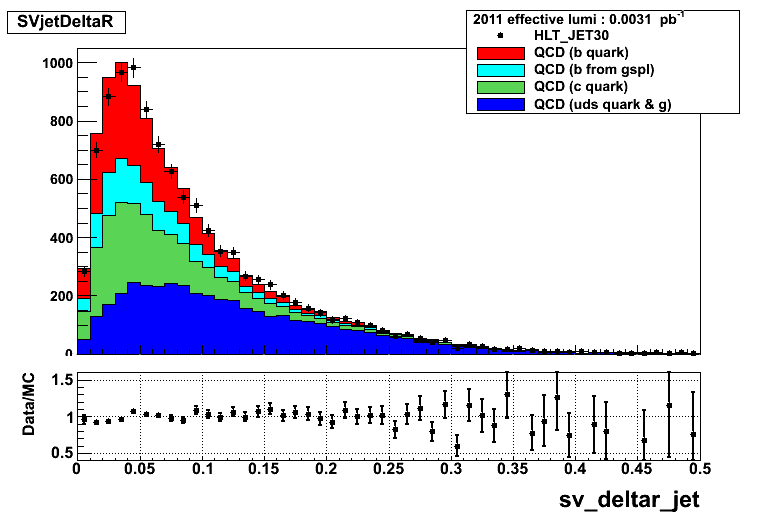
\includegraphics[width=0.32\textwidth]{figures/HLTJet30sv_deltar_jet_Linear.png}
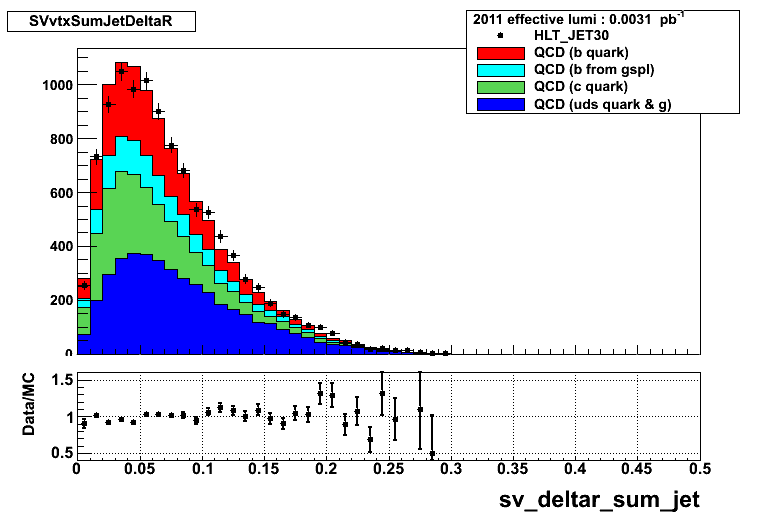
\includegraphics[width=0.32\textwidth]{figures/HLTJet30sv_deltar_sum_jet_Linear.png}
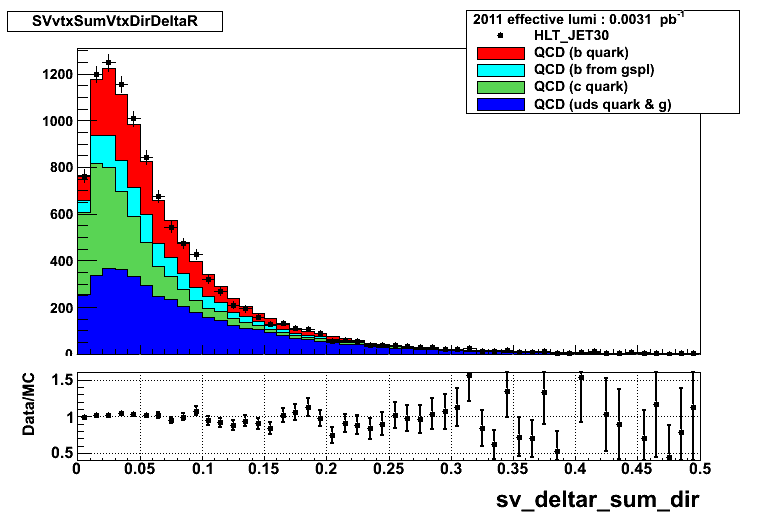
\includegraphics[width=0.32\textwidth]{figures/HLTJet30sv_deltar_sum_dir_Linear.png}
\caption{Left: angular distance in $\Delta R$ between jet axis and vertex direction. Middle: angular distance in $\Delta R$ between jet axis and the sum of track momenta at the vertex, Right: angular distance in $\Delta R$ between vertex direction and the sum of track momenta at the vertex. }
\label{fig:HLTJet30vertexAngles}
\end{figure}

\begin{figure}[h!]
\centering
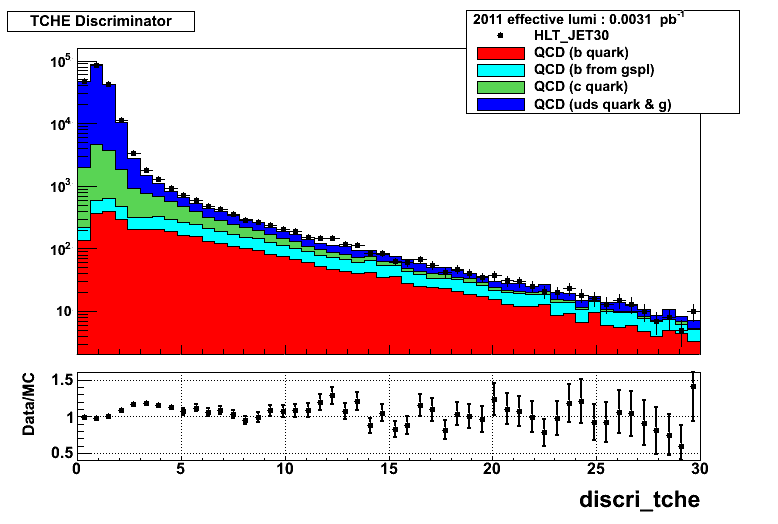
\includegraphics[width=0.45\textwidth]{figures/HLTJet30discri_tche_Log.png}
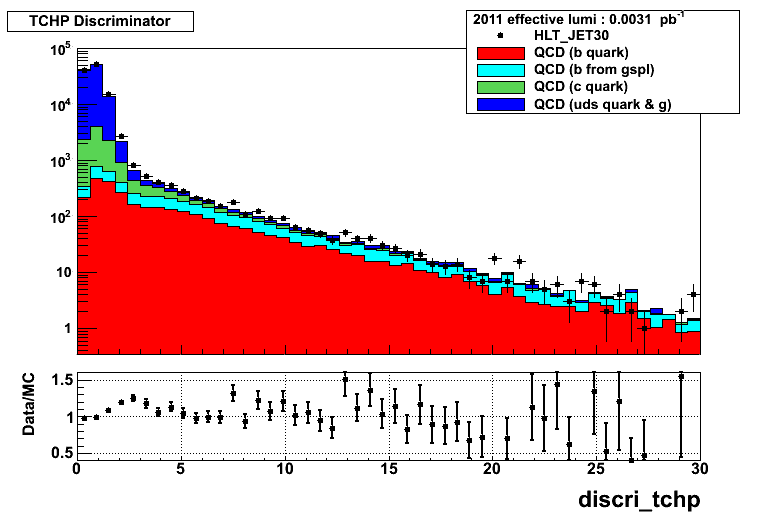
\includegraphics[width=0.45\textwidth]{figures/HLTJet30discri_tchp_Log.png}
\caption{Left: track counting high efficiency, Right: track counting high purity discriminators. }
\label{fig:HLTJet30trackCountingDisc}
\end{figure}
\begin{figure}[h!]
\centering
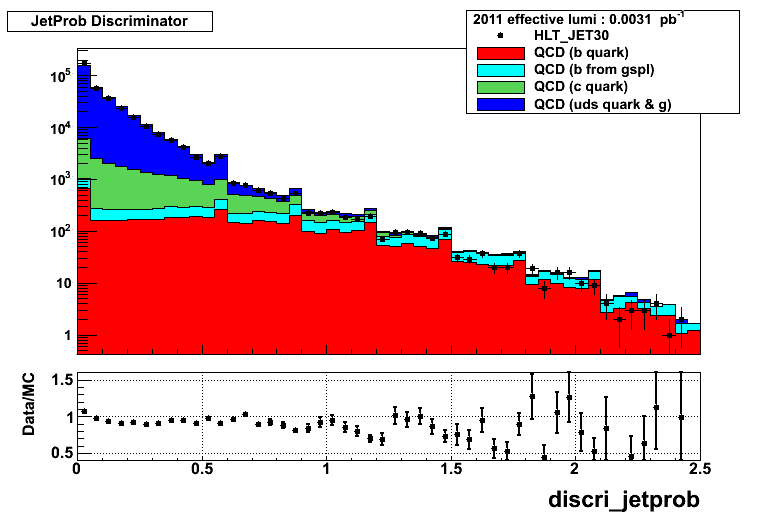
\includegraphics[width=0.45\textwidth]{figures/HLTJet30discri_jetprob_Log.png}
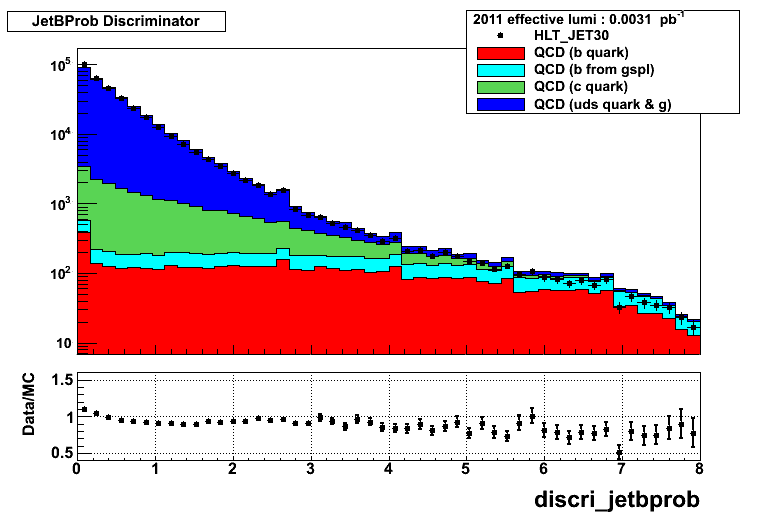
\includegraphics[width=0.45\textwidth]{figures/HLTJet30discri_jetbprob_Log.png}
\caption{Left: jet probability , Right: jet B probability discriminators. }
\label{fig:HLTJet30JetProbDisc}
\end{figure}
\begin{figure}[h!]
\centering
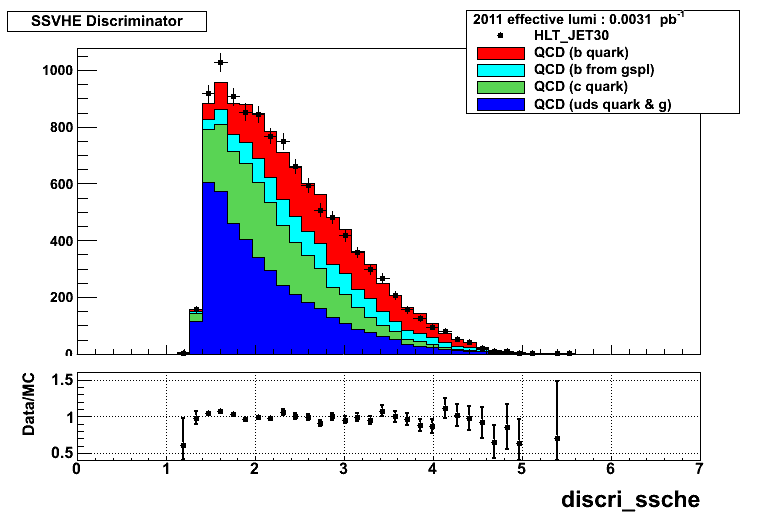
\includegraphics[width=0.45\textwidth]{figures/HLTJet30discri_ssche_Linear.png}
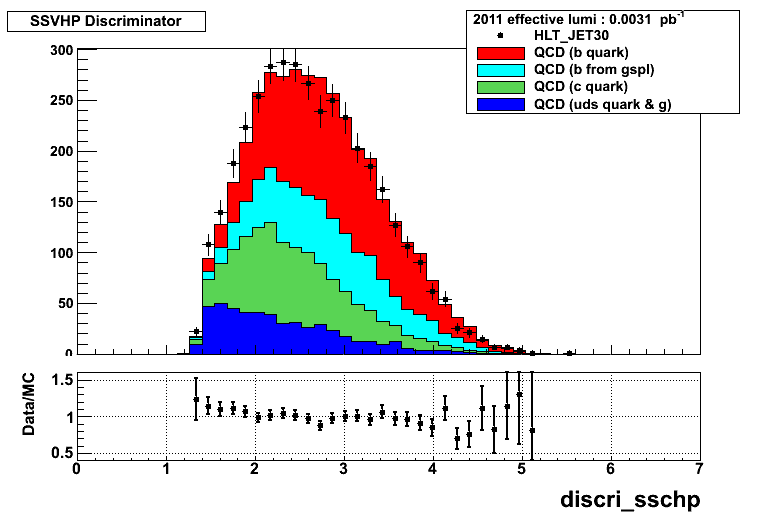
\includegraphics[width=0.45\textwidth]{figures/HLTJet30discri_sschp_Linear.png}
\caption{Left: simple secondary vertex high efficiency , Right: simple secondary vertex high purity discriminators. The underflow bin for jets which do not contain a reconstructed secondary vertex is not displayed.}
\label{fig:HLTJet30SimpleSVDisc}
\end{figure}

\begin{figure}[h!]
\centering
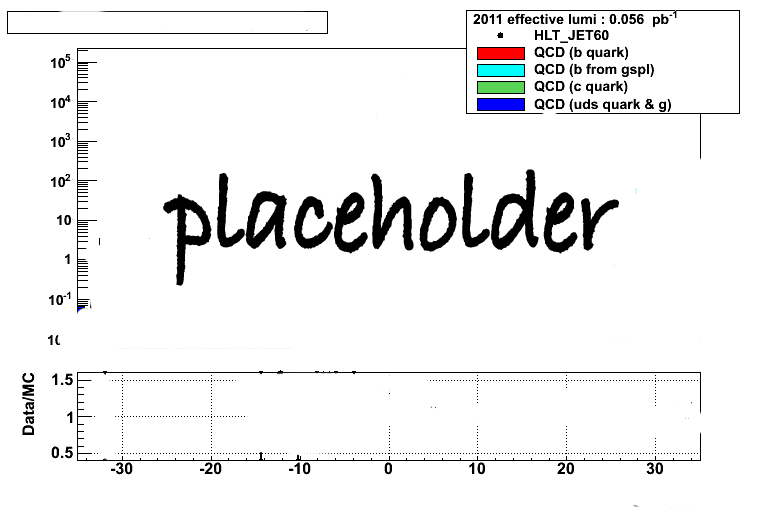
\includegraphics[width=0.45\textwidth]{figures/placeholder.png}
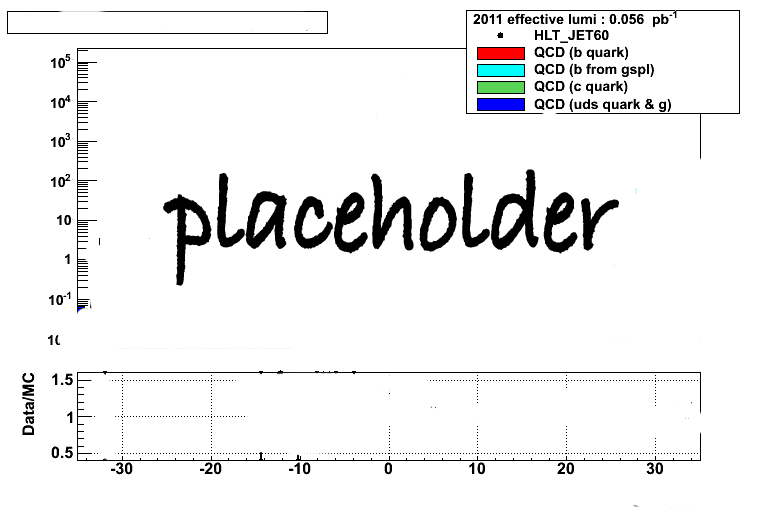
\includegraphics[width=0.45\textwidth]{figures/placeholder.png}
\caption{Left: track counting high efficiency tagging rate, Right: track counting high purity tagging rate. }
\label{fig:HLTJet30trackCountingDiscEff}
\end{figure}
\begin{figure}[h!]
\centering
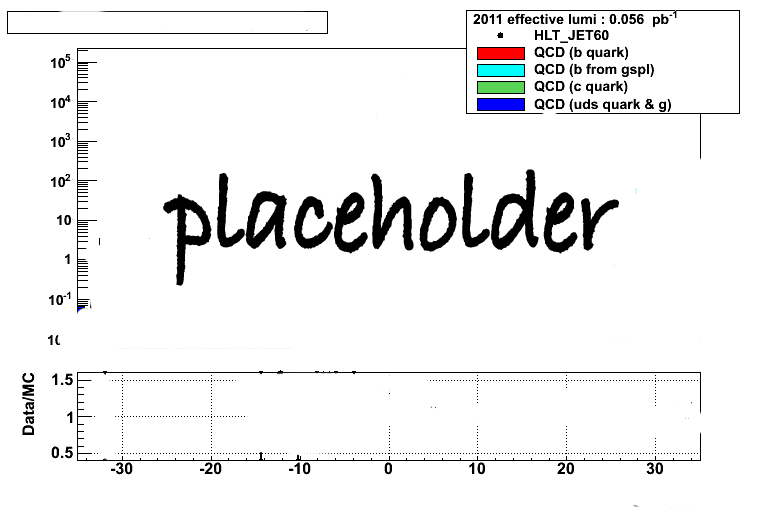
\includegraphics[width=0.45\textwidth]{figures/placeholder.png}
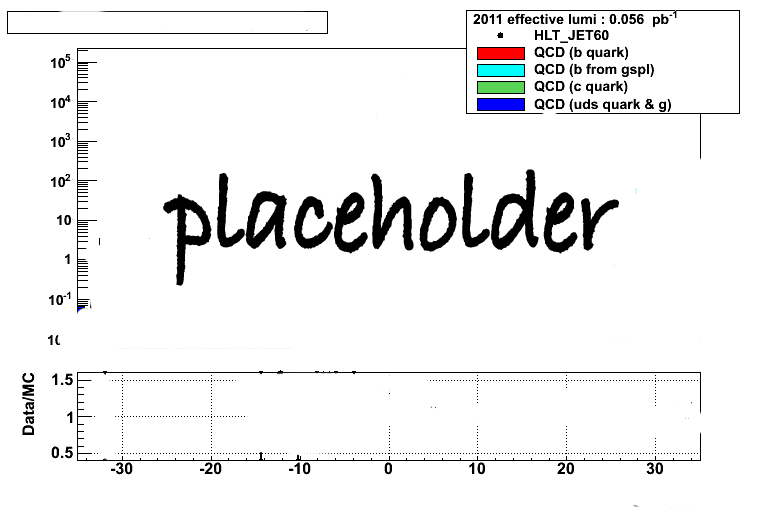
\includegraphics[width=0.45\textwidth]{figures/placeholder.png}
\caption{Left: jet probability tagging rate, Right: jet B probability tagging rate. }
\label{fig:HLTJet30JetProbDiscEff}
\end{figure}
\begin{figure}[h!]
\centering
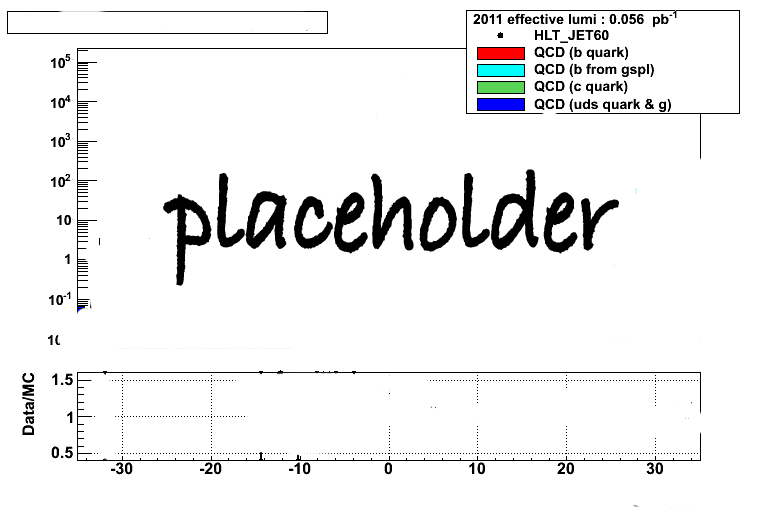
\includegraphics[width=0.45\textwidth]{figures/placeholder.png}
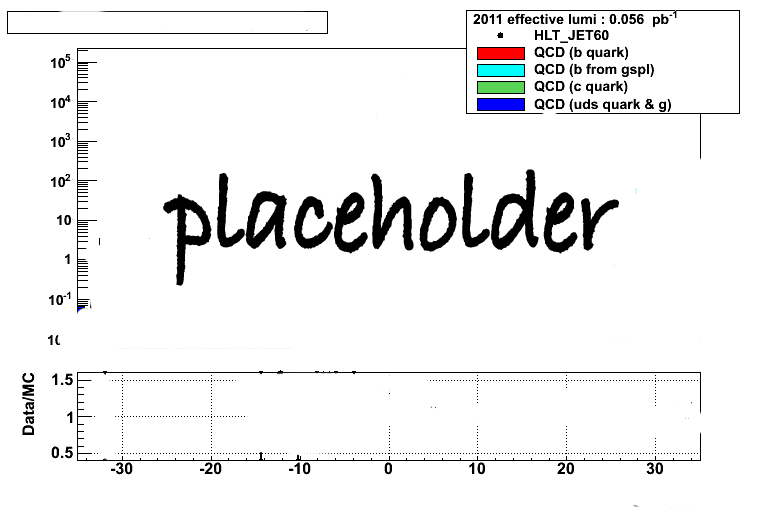
\includegraphics[width=0.45\textwidth]{figures/placeholder.png}
\caption{Left: simple secondary vertex high efficiency tagging rate, Right: simple secondary vertex high purity tagging rate. }
\label{fig:HLTJet30SimpleSVDiscEff}
\end{figure}

\begin{figure}[h!]
\centering
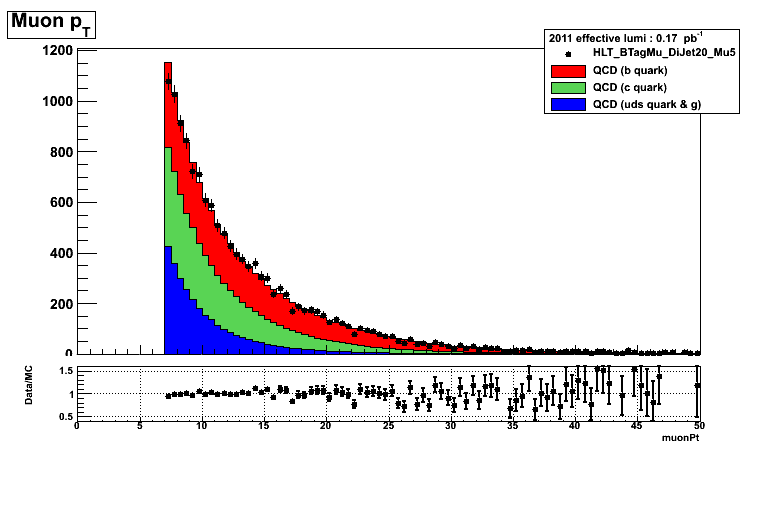
\includegraphics[width=0.32\textwidth]{figures/HLTbtagmu_dijet20mu5mujetmuonPt_Linear.png}
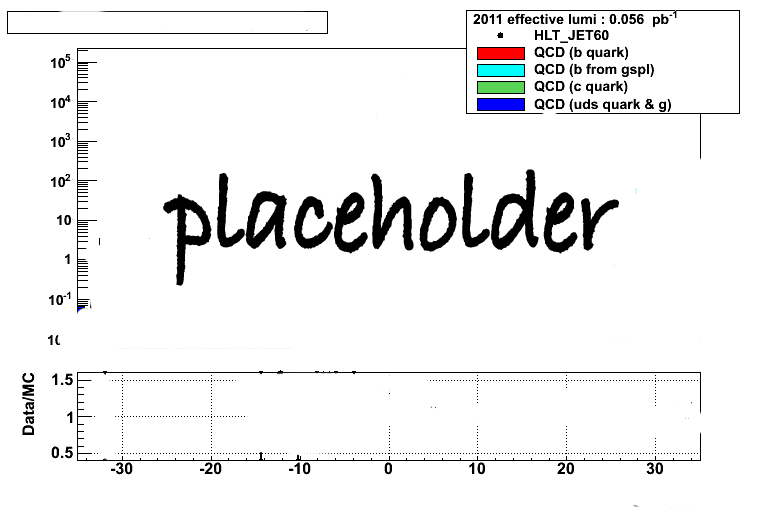
\includegraphics[width=0.32\textwidth]{figures/placeholder.png}
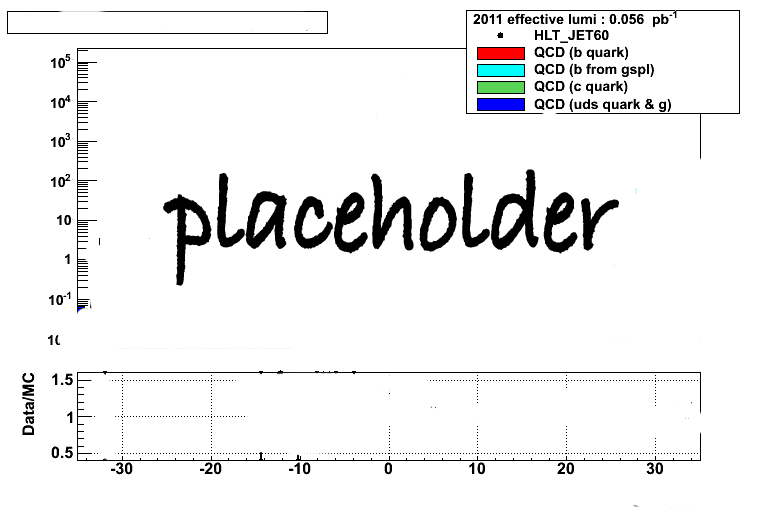
\includegraphics[width=0.32\textwidth]{figures/placeholder.png}
\caption{Left: transverse momentum $p_t$ of muons in jets. Middle: number of reconstructed muons per jet. Right: 3D impact parameter significance of muons in jets.}
\label{fig:HLTJet30muonplots1}
\end{figure}


\begin{figure}[h!]
\centering
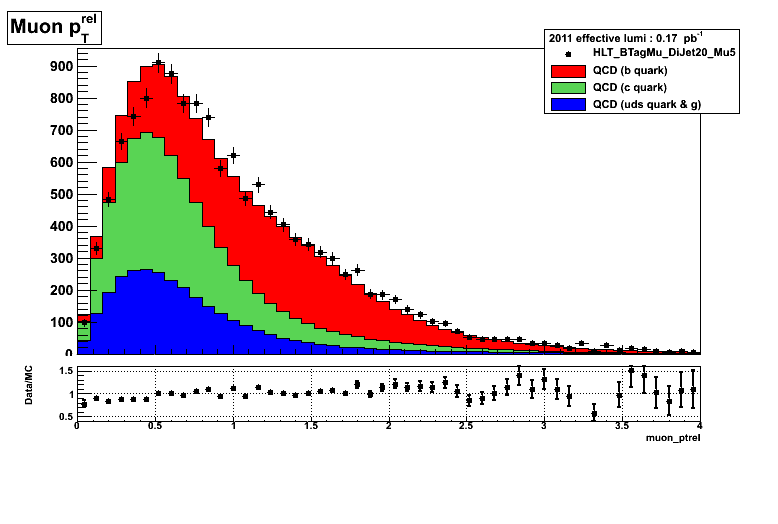
\includegraphics[width=0.42\textwidth]{figures/HLTbtagmu_dijet20mu5mujetmuon_ptrel_Linear.png}
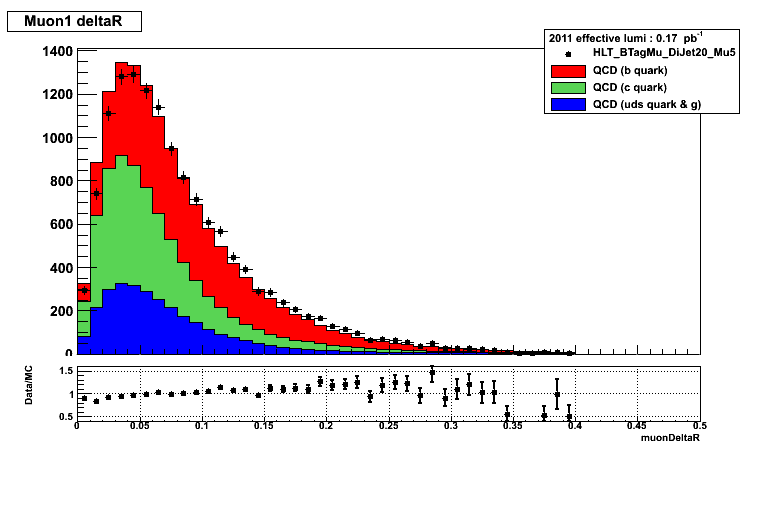
\includegraphics[width=0.42\textwidth]{figures/HLTbtagmu_dijet20mu5mujetmuonDeltaR_Linear.png}
\caption{Left: transverse momentum of the muon with respect to the jet axis $p_t^{rel}$. Right: angle (in units of $\Delta R$) between the muon and the jet axis.}
\label{fig:HLTJet30muonplots2}
\end{figure}

\begin{figure}[h!]
\centering
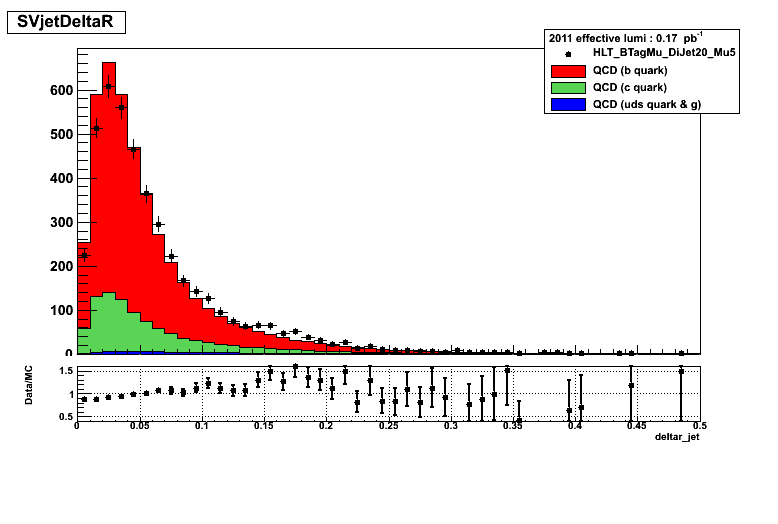
\includegraphics[width=0.32\textwidth]{figures/HLTbtagmu_dijet20mu5mujetsv_deltar_jet_Linear.png}
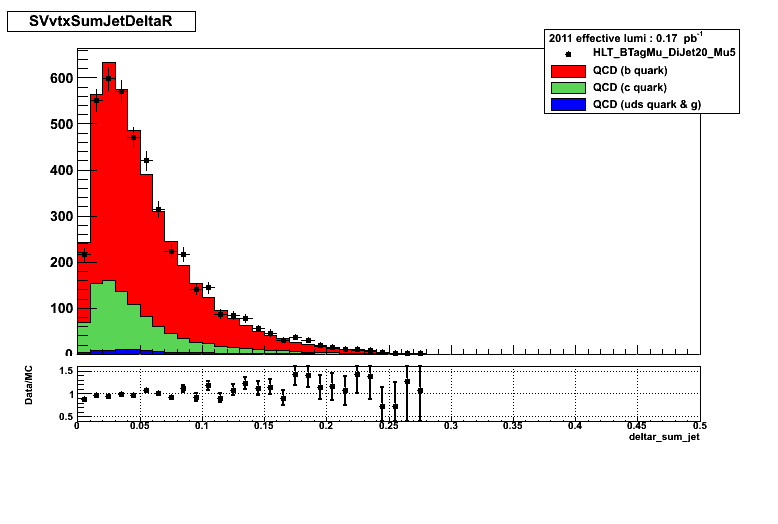
\includegraphics[width=0.32\textwidth]{figures/HLTbtagmu_dijet20mu5mujetsv_deltar_sum_jet_Linear.png}
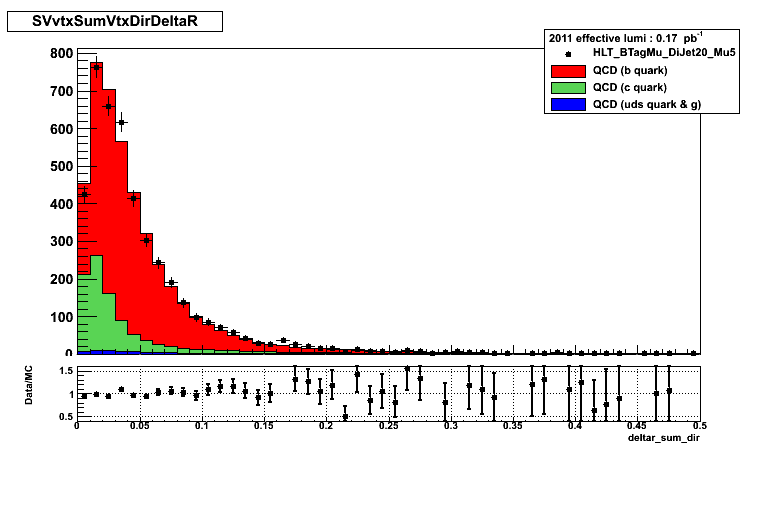
\includegraphics[width=0.32\textwidth]{figures/HLTbtagmu_dijet20mu5mujetsv_deltar_sum_dir_Linear.png}
\caption{Left: angular distance in $\Delta R$ between jet axis and vertex direction. Middle: angular distance in $\Delta R$ between jet axis and the sum of track momenta at the vertex, Right: angular distance in $\Delta R$ between vertex direction and the sum of track momenta at the vertex. }
\label{fig:HLTJet30vertexAnglesMuJets}
\end{figure}